\documentclass{article}
%\usepackage[latin1]{inputenc}
\usepackage{graphicx,amssymb,amsmath,amsbsy,MnSymbol} % extensions pour maths avancées
\usepackage{graphicx}           % extensions pour figures
\usepackage[T1]{fontenc}        % pour les charactères accentués 
\usepackage[utf8]{inputenc} 

\usepackage{stmaryrd} % Pour les crochets d'ensemble d'entier
\usepackage{float}  % Pour placer les images là ou JE veux.

\DeclareMathOperator{\tr}{tr}
\DeclareMathOperator{\argmax}{argmax}


\setlength{\parindent}{0.0in}
\setlength{\parskip}{0.3in}
\setlength{\topmargin}{-0.4in}
\setlength{\topskip}{1in}    % between header and text
\setlength{\textheight}{8in} % height of main text
\setlength{\textwidth}{4.5in}    % width of text
\setlength{\oddsidemargin}{1in} % odd page left margin
\setlength{\evensidemargin}{1in} % even page left margin
%
%% Quelques raccourcis clavier :
\def\slantfrac#1#2{\kern.1em^{#1}\kern-.3em/\kern-.1em_{#2}}
\def\b#1{\mathbf{#1}}
\def\bs#1{\boldsymbol{#1}}
\def\m#1{\mathrm{#1}}
%
\newcommand{\greeksym}[1]{{\usefont{U}{psy}{m}{n}#1}}
\newcommand{\inc}{\mbox{\small\greeksym{d}\hskip 0.05ex}}%
\pagenumbering{arabic}
\date{\today}
\title{DM2: Modèles Graphiques}
\author{Barbara Gris \& Nelle Varoquaux}
\begin{document}
\maketitle
\tableofcontents{}
\vfill \eject

\section{Distributions factorisables dans un graphe}
\subsection{Question a}

Soit $G = (V, E)$ et soit $i \rightarrow j$ une arête couverte, i.e, telle que
$\pi_j = \pi_i \bigcup \{i\}$.
Soit $G'= (V,E)$, avec $E' = (E \setminus \{i \rightarrow j\}) \bigcup \{j \rightarrow i\}$.

Montrons que $\mathcal{L}(G) = \mathcal{L}(G')$


Par définition, on a:
\begin{align}
\mathcal{L}(G) & = & \{ p \mid p(x) = \prod_{k = 1}^{n} p(x_k \mid x_{\pi_k}) \} \\
	       & = & \{ p \mid p(x) = A p(x_i \mid x_{\pi_i}) p(x_j \mid x_{\pi_j} \}
\end{align}

avec $A = \prod_{k \in V \setminus \{i, j\} p[x_k \mid x_{\pi_k}]}$. De même, on a:

\begin{align}
\mathcal{L}(G') & = & \{ p \mid p(x) = \prod_{k = 1}^{n} p(x_k \mid x_{\pi'_k}) \} \\
		& = & \{ p \mid p(x) = A p(x_i \mid x_{\pi'_i}) p(x_j \mid x_{\pi'_j} \}
\end{align}

De plus,

$$\pi_j = \pi_i \bigcup \{ i \}$$
$$\pi'_j = \pi_j \setminus \{ i \} = \pi_i$$
$$\pi'_i = \pi_i \bigcup \{ j \}$$

On peut donc écrire $(4)$ comme:
\begin{align}
\mathcal{L}(G') & = & \{ p \mid p(x) = A p(x_i \mid x_{\pi_i \bigcup \{ j \}}) p(x_j \mid x_{\pi_i} )\} \\
		& = & \{ p \mid p(x) = A p(x_i \mid x_{\pi_i}, x_j) p(x_j \mid x_{\pi_i})\}
\end{align}

En posant $q = p(. \mid x_{\pi_i})$, on a par la formule de Bayes $q(x_i)q(x_j \mid x_i) =  q(x_j)q(x_i \mid x_j)$.
D'où $p(x_j \mid x_{\pi_i})p(x_i \mid x_{\pi_i}, x_j) = p(x_i \mid x_{\pi_i})p(x_j \mid x_{\pi_i}, x_i)$. Donc

\begin{align}
\mathcal{L}(G') & = & \{ p \mid p(x) = A p(x_i \mid x_{\pi_i}) p(x_j \mid x_{\pi_i}, x_i) \\
	        & = & \{ p \mid p(x) = A p(x_i \mid x_{\pi_i}) p(x_j \mid x_{\pi_i \bigcup \{i\}} \} \\
		& = & \{ p \mid p(x) = A p(x_i \mid x_{\pi_i}) p(x_j \mid x_{\pi_j}) \\
		& = & \mathcal{L}(G)
\end{align}


\subsection{Question b}

\begin{figure}[h]
  \caption{Graphe 1}
  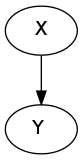
\includegraphics[width=30px]{1.png}
\end{figure}

Soit un graphe non orienté $G$ à deux nœuds. Le graphe (1) factorise toutes
les lois sur deux variables aléatoires. En effet pour toute loi $p$ sur deux
variables aléatoires $X$ et $Y$, $p(x,y)=p(x)*p(x|y)$ et donc $p$ se factorise
bien dans $G'$. Ainsi toute loi sur $X$,$Y$ se factorise dans $G'$ i.e. comme
$\mathcal{L}(G)$ est l'ensemble des lois sur deux variables aléatoires,
$\mathcal{L}(G)=\mathcal{L}(G')$.

\begin{figure}[h]
  \caption{Graphe 2}
  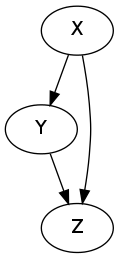
\includegraphics[width=30px]{2.png}
\end{figure}


Soit $G$ un graphe non orienté à trois nœuds. Un graphe orienté à trois nœuds
est forcément de la forme (2) car on exclue le cas où il y a des cycles. Soit
une loi quelconque $p$ sur trois variables aléatoires $X$, $Y$, et $Z$. On a
de manière générale $p(x,y,z) = p(x)*p(y|x)*p(z|x,y)$ et donc cette loi se
factorise bien dans $G'$. Ainsi de même que précédemment,
$\mathcal{L}(G)=\mathcal{L}(G')$.

\begin{figure}[h]
  \caption{Graphe 3}
  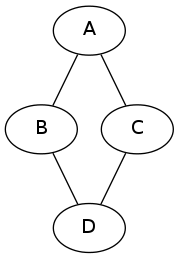
\includegraphics[width=30px]{3.png}
\end{figure}

Soit alors $G$ (3). Soit $G'$ un graphe orienté à quatre nœuds. Si $G'$ est
une chaîne (5) alors il y a forcément une indépendance de deux variables
aléatoires conditionnellement à une seule des deux autres ce qui n'est pas le
cas dans $G$ donc $\mathcal{L}(G) \neq \mathcal{L}(G')$. Si les arêtes de $G'$
sont les mêmes que celles de $G$, il y a forcément une structure en v en un
nœud $X$ car on exclue le cas où il y a des cycles et il y a de même forcément
un nœud $Y$ sans parents. Il y a trois situations possibles:

\begin{itemize}
  \item graphe (4a) : on a la contrainte d'indépendance $B \upmodels C \mid D$
  car $D$ d-sépare $B $ et $C$.
  \item graphe (4b) :on a la contrainte d'indépendance $A \upmodels D \mid B$
  car $B$ d-sépare $A$ et $C$.
  \item graphe (4c) : on a la contrainte d'indépendance $B \upmodels C$ car
  l'ensemble vide d-sépare $A$ et $D$.
\end{itemize} 

Ces contraintes ne sont pas vraies pour $G$ donc dans chaque cas
$\mathcal{L}(G) \neq \mathcal{L}(G')$.

Si l'on rajoute une arête à l'un des graphes précédents, on perd l'une des
contraintes $A \upmodels D \mid B,C$ et $B \upmodels C \mid A,D$ imposées par
le graphe $G$ donc $\mathcal{L}(G) \neq \mathcal{L}(G')$.

Ainsi il n'existe pas de graphe orienté $G'$ tel que $\mathcal{L}(G) =
\mathcal{L}(G')$ et $G$ est le plus petit graphe vérifiant cette propriété.

\begin{figure}[h]
\caption{Graphe non orienté $G$}
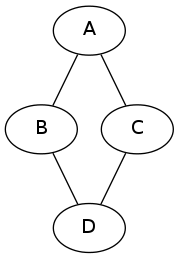
\includegraphics[width=100px]{Ia.png}
\end{figure}

\section{d-Séparation}

\subsection{Question a}

Soit $G$ un DAG et $G_M$ le graphe moralisé. Soient $A$, $B$ et $S$ trois
ensembles de nœuds disjoints tels que $A$ et $B$ soient séparés par $S$ dans
$G_M$. Montrons que $A$ et $B$ sont d-séparés par $S$ dans $G$.

Soit $c = (v_{1}, ..., v_{n})$ une chaîne de $G$ telle que $v_{1} \in A$ et
$v_{n} \in B$. On construit une chaîne $\tilde{c}$ de $G_M$ telle que tout
nœud de $\tilde{c}$ est un nœud $v_i$ de $c$ tel que $v_{i-1},v_{i},v_{i+1}$
ne forme pas une structure en $v$ :

\begin{itemize}
  \item On part de $\tilde{c}=(v_{1})$.
  \item Pour  $i$ allant de 2 à $n-1$, si $v_i$ est tel que
  $v_{i-1},v_{i},v_{i-1}$ n'est pas une structure en v, on ajoute $v_i$ à
  $\tilde{c}$; sinon on ne l'ajoute pas.
  \item Pour finir, on ajoute $v_{n}$. 
\end{itemize}

Ainsi $\tilde{c} = (c_{1}, ..., c_{d})$ avec $c_1 = v_1$, $c_d = v_n$ et
$\forall i \in \{1,...,d-1\}$, $\exists j \in \{1,...,n-1\}$ tel que $c_i =
v_j$ et 

\begin{itemize}
  \item soit $c_{i+1} = v_{j+1}$, donc $(c_{i},c_{i+1})=(v_{i},v_{i+1})$ est
  une arête de $G_M$ et $v_{i},v_{i+1},v_{i+2}$ n'est pas une structure en v;
  \item soit $c_{i+1} = v_{j+2}$ et $v_{i},v_{i+1},v_{i+2}$ est une structure
  en v. Dans ce cas, $v_{i}$ et $v_{i+2}$ sont des parents de $v_{i+1}$ donc
  $(v_{i},v_{i+2})=(c_{i},c_{i+1})$ est une arête de $G_M$.
\end{itemize}

Ainsi on a bien construit la chaîne $\tilde{c}$ comme on le voulait. Comme
c'est une chaîne dans $G_M$ qui va de $A$ à $B$, il existe un nœud de cette
chaîne qui est dans $S$. Alors il existe $i\in \{2,...,n-1\}$ tel que ce nœud
est $v_i$ et de plus par construction $v_{i-1},v_{i},v_{i-1}$ n'est pas une
structure en c. Ainsi $S$ bloque la chaîne $c$. Finalement, $S$ d-sépare bien
$A$ et $B$.


\subsection{Question b}

Cette assertion est fausse, en effet le graphe suivant la contredit.

\begin{figure}[h]
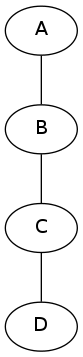
\includegraphics[width=100px]{5.png}
\end{figure}


\subsection{Question c}

\begin{itemize}
\item L'assertion $X_{\{1, 2\}} \upmodels X_4 \mid X_3$ est fausse: ${1, 8, 4}$ n'est pas
bloqué par $4$.
\item L'assertion $X_{\{1, 2\}} \upmodels X_4 \mid X_5$ est fausse: le chemin précédant
n'est pas bloqué par $5$.
\item L'assertion $X_1 \upmodels X_6 \mid X_{\{2, 4, 7\}}$ est vraie. Tous les chemins
de $1$ vers $6$ sont bloqués par $7$.
\end{itemize}


\end{document}
